\documentclass{article}
\title{Bear Grylls Project \\ \large  Using deep reinforcement learning to create an agent able to survive in a hostile environment.}
\author{Erwan Simon}
\usepackage{hyperref}
\usepackage{graphicx}
\begin{document}

\maketitle

\tableofcontents

\newpage

\section{Abstract}

\paragraph{•}
We present a world suited to test the capacity of an agent to harvest resources at a minimum speed. It has to navigate around obstacles which interfer with its progression, all of that with limited vision of its environment. An agent enable to maintain a minimal harvesting speed dies.\par
We also provide a description of our tries to implement an algorithm of deep reinforcement learning which can answer to this task in the most efficient way possible.\par

\section{Introduction}

\paragraph{Reinforcement learning}
(RL) is a cutting-edge field in unsupervised learning. Some recent work showed its potential to resolve many complexe problems and beat human expertise in some trivial domains\cite{DBLP:journals/corr/MnihKSGAWR13} and some less trivial ones\cite{healthcare}. The relative earliness of this field may be the cause explaining why it has so much unsolved (or partially solved) problematics among which we can find delayed reward, progression in partially visibe environment (also called non-Markovian decision problem)\cite{bakker2002reinforcement} and generalization to previously unseen situations\cite{sutton1996generalization}.

\paragraph{Deep learning}
has proven to be a good way to improve RL policy (reference needed). Indeed, deep neural networks and their capacities to approximate complexe functions are an excellent tool to represent and perfectionnate the existing links between a state and the result of a action on this state. There is not so much work done in this area relatively speaking compared to other deep learning fields. This could be explain by the fact that reinforcement learning is an ungrateful domain if not deeply uneffective\cite{rlblogpost}. We don't expect here any ground breaking progress considering this paper is more of a domain explorer than a state-of-the-art maker.

\paragraph{The game}
we are presenting here is a solution to test several of the above presented problems. The agent has a limited view of its environment (whence the non-Markovian problem). A reasonably big map paired with random apparition location of the map's features implies that the agent cannot overfit the disposition of its environment, which allow us to test its generalization abilities. Finally, the sparse resources on the map brings the delayed reward problematic. All of this to state that this game is perfect to train deep reinforcement learning agents and test their abilities to survive in hostile environment.

\paragraph{The general hypothesis}
here is that a deep reinforcement learning agent trained with effective parameters can successfully answer the problematics presented above.

\section{Methods}

\subsection{The game}

\subsubsection{The environment}

\paragraph{The board}
is composed by a two-dimensionnal discrete toric world made of squares (technical jargon to say we have a grid where if an agent exists by one side of the board it will come back through the opposit side). More concrete representation can be found in Figure 1.

\begin{figure}
\centering
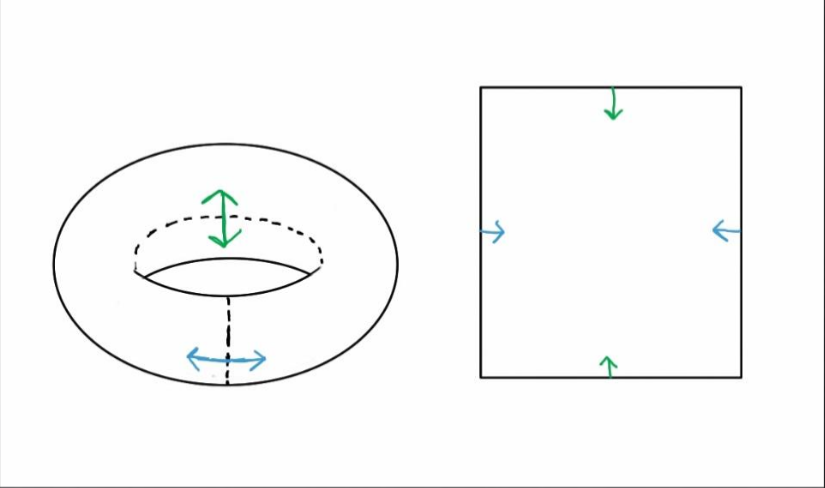
\includegraphics[scale=0.2]{toric_world.png}
\caption{Visual representation of a toric world}
\end{figure}

\paragraph{The food}
appears at random location of the board. It grants extra surviving time to agents. The extra time given by one food can be changed to modify the experiment. Raise its value garrantees that agents will have more time before starving to death. If an agent walks on a tile with a food on it, food is transfered to agent inventory and disappears from the tile. Another food then appears in a random location of the board.

\paragraph{Obstacles}
appear at the initial creation of the board and their location never change. Percentage of obstacles compared with total number of tile on the board can be set. More obstacles implies more difficulty for an agent to wander around. If an agent try to go on a tile with a trap in it, it just do not move and stays on the tile it was on.

\paragraph{Stones}
spawn at random location on the board. If an agent walks on a stone, it picks it and adds it in its inventory. There can be only a limited setable number of stone on the board and in the inventories of agents. Therefore, stones only appears on the board at the begining of the board and when an agent possessing a stone dies. This implies a notion of scarcity of this resource. \par
It does not stricly speaking have any use for an agent to pick a stone yet. Maybe in the future we could imagine a notion of level which could be increased depending on the number of stone possessed by an agent.

\subsubsection{The agent}

\paragraph{•}
An agent appears at a random location of the board (location which cannot contain a obstacle) at the begining of the game and when it dies (from starvation). \par

\paragraph{•}
Inventory of the agents have an amount of food and an amount of stones.

\paragraph{•}
Agents have to move one tile at a time up, down, left or right every turn. They also have a stealing action which if used when in the same tile of another agent which possesses a stone, steals this stone and adds it to the stealer inventory.

\paragraph{•}
Agents have a limited sight of their environment, which wideness is setable. Setting it higher allows them to have a better view on what is around them but it also makes the enviromnent more complexe in their eyes.

\subsection{The experiment}

\subsubsection{Reinforcement learning}

Reinforcement learning's different algorithms always have three main parts : the state, the reward and the policy.

\paragraph{The state}
contains the vision of the agent with the surrounding tiles, which allow it to locate food, obstacles and stones. \par
It also contains the current food amount of the agent and the number of stones it possesses. \par
The state is litterally the only mean for the agent to see its surrounding.

\paragraph{The reward}
allows us to say to the agent if something is good or bad. I.E. dying is bad and eating food is good.\par 
Finding the right reward system is very important as well as very difficult. Indeed, a too much explicite one could be considered as cheating because we can no longer consider that the agent discovers the rules of the game by itself. A reward to vague and our agent will not be able to learn anything.\par 
The equilibrium is a vital aspect too. A too punitive reward system could lead to problematic behaviour such as learned helpnessness\cite{wiki:learned_helplessness}. This behaviour leads to unsatisfactory results, like the agent juste going around in circle.\par
It is also very important to not give an either positive nor negative reward if there is not any change in the state, because it encourages the choice of random decisions by the agent (or at least a decision based on wrong inferences).

\paragraph{The policy}
is the action taken by the agent depending on the current state and the desired state. The main principle of reinforcement learning is to improve the policy tu ensure that the agent will make a decision depending of the state. A good policy improvement eventually ensures that the choice of an action will lead to the maximum possible reward in the medium term (or in the short one).

\paragraph{•}
The referencial reinforcement learning algorithms used in this paper are Q-Learning\cite{watkins1992q} and Temporal Difference learning (TD)\cite{tsitsiklis1997analysis}.

\subsubsection{Deep learning}

The optimisation of the policy can be made thanks to deep neural networks. 

\section{Results}

\section{Discussion}

\bibliographystyle{unsrt}
\bibliography{sources}

\end{document}